
\documentclass{sig-alternate}
\usepackage[normalem]{ulem}
\usepackage[usenames,dvipsnames]{pstricks}

\usepackage{mathtools}

\usepackage{algorithm2e}



\usepackage{multirow}

\begin{document}
\conferenceinfo{CIKM}{'13 Burlingame, California USA}
\title{Efficient Temporal Synopsis of Social Media Streams}

\maketitle
\begin{abstract}
Search and summarization of streaming social media, such as Twitter, requires the ongoing analysis of large volumes of data with dynamically changing characteristics.  tweets are short and repetitious - lacking context and structure  - making it difficult to generate a coherent synopsis of events within a given time period.  Although some established algorithms for frequent itemset analysis might provide an efficient foundation for synopsis generation, the unmodified application of standard methods produces a complex mass of rules, dominated by common language constructs and many trivial variations on topically related results.  Moreover, these results are not necessarily specific to events within the time period of interest.  To address these problems, we build upon the Linear time Closed itemset Mining (LCM) algorithm, which is particularly suited to the large and sparse vocabulary of tweets.  LCM generates only closed itemsets, providing an immediate reduction in the number of trivial results.  To reduce the impact of function words and common language constructs, we apply a filtering step that preserves these terms only when they may form part of a relevant collocation.  To further reduce trivial results, we propose a novel strengthening of the closure condition of LCM to retain only those results that exceed a threshold of distinctiveness.  Finally, we perform temporal ranking, based on information gain, to identify results that are particularly relevant to the time period of interest.  We evaluate our work over a collection of tweets gathered in late 2012, exploring the efficiency and filtering characteristic of each processing step, both individually and collectively.  Based on our experience, the resulting synopses from various time periods provide understandable and meaningful pictures of events within those periods, with potential application to tasks such as temporal summarization and query expansion for search.
\end{abstract}
%\category{H.4}{Information Systems Applications}{Miscellaneous}
%A category including the fourth, optional field follows...
%\category{D.2.8}{Software Engineering}{Metrics}[complexity measures, performance measures]

%\terms{Theory}

%\keywords{ACM proceedings, \LaTeX, text tagging}
\newpage
\section{Introduction}

The nature of text in social media poses a challenge when applying
traditional text mining algorithms.
Text in social media is usually short, lacks context and structure,
and is created at a very high rate.
To realize the benefits of social media in giving a voice to ordinary people,
this work focuses on the content of posts.
However, the collective stream from all users is overwhelmed with personal
updates, and timely finding posts about topics of interest requires an
efficient mining algorithm.
The frequent itemset mining family of algorithms is fast and efficient,
however it is not readily suited for application on text.
First, the number of itemsets mined is large and grows with the number of
distinct items~---~which is particularly high in the text domain.
Frequent itemset mining was originally proposed as a preliminary stage for
association rules mining, which sifts through the numerous itemsets and
produces a smaller number of association rules.
To reduce the number of itemsets, they may be limited by setting a high
frequency threshold, but this is not possible in text mining because
frequencies of items follow a long-tailed Zipfean distribution.
Second, the high frequency of stop words and language constructs is a problem
that frequent itemset mining is not equipped to handle.
Even if a maximum frequency threshold is set, incurring the risk that we
will filter out important itemsets, many of non-English constructs will be
mined because the proportion of posts in English is much higher than
other languages.  Finally, there is considerable redundancy in frequent
itemsets caused by trivial differences in the language used.
In this paper we address those problems, adapting frequent itemset mining to
social media text without degrading its efficiency.

Unlike trending
topics\footnote{http://blog.twitter.com/2010/12/to-trend-or-not-to-trend.html}
\cite{mathioudakis2010twittermonitor}, the results of frequent itemset
mining includes itemsets that have high frequency because of sustained interest,
as well as a spike of interest.
The mined itemsets provide the vocabulary associated with events and can be
used as a preliminary step for search and summarization.
For example, the collection of mining results from different epochs of time
can be used for temporal query and document
expansion~\cite{choi2012temporal, efron2012improving}.
The results from each epoch can be treated as a document, facilitating the
creation of a ``temporal profile''\cite{jones2007temporal} of the query
or a document being expanded.
For summarization, frequent itemsets can provide a good foundation for summary
creation.
While the frequent itemsets themselves are not summaries, since they lack
qualitative properties such as coherence and cohesion, the results are
unstandable at the user level.
As we shall see in later examples, the top ranked itemsets cover a variety
of open topics, and within one topic different opinions are reported as
separate contrastive itemsets.

The next three sections provide necessary background.
We start by discussing related work in section \ref{sec:related},
we then explain frequent itemset mining and the algorithm on which we build
our work in sections \ref{sec:fim} and \ref{sec:lcm} respectively.
In sections \ref{sec:socmine}, \ref{sec:strong} and \ref{sec:rank} we
propose solutions to different problems faced when applying frequent
itemset mining to social media text.
We present the outline of those sections graphically using a
frequency ordered prefix tree of the itemsets.
Each path from root to a leaf in such a tree represents an itemset,
where each itemset is ordered in non-increasing order of the frequency of
items.
Itemsets having the same prefix share the nodes representing this prefix.
This representation is typical in the literature, and it is actually a very
good representation of the frequent itemset mining problem.
Figure \ref{fig:outline} shows conceptually how our contributions in sections  \ref{sec:socmine},
\ref{sec:strong} and \ref{sec:rank}  affects different parts of the
problem. We overlay the contributions on such a figure to make it clear how each one addresses a particular challenge of applying frequent itemset mining to text data from social media. In section \ref{sec:concfut}, we conclude our presentation and
suggest future directions.

\begin{figure*}
\centering
\scalebox{0.7} 
{
\begin{pspicture}(0,-4.41)(17.948048,4.4013004)
\pstriangle[linewidth=0.04,dimen=outer](8.617168,-4.41)(17.14,8.82)
\psline[linewidth=0.04cm](0.827168,-3.59)(16.367168,-3.61)
\psline[linewidth=0.04cm,linestyle=dashed,dash=0.16cm 0.16cm](6.927168,2.57)(10.287168,2.59)
\usefont{T1}{ptm}{m}{n}
\rput(8.60748,-4.005){Items with low frequency in the data are excluded by frequent itemset mining, and hence not part of the tree}
\psline[linewidth=0.04cm,linestyle=dashed,dash=0.16cm 0.16cm](2.487168,-2.03)(14.8271675,-2.01)
\usefont{T1}{ptm}{m}{n}
\rput(3.4739747,4.075){The top of the tree is not as small as it seems.}
\usefont{T1}{ptm}{m}{n}
\rput(3.6774805,3.655){It contains a large number of itemsets which are}
\usefont{T1}{ptm}{m}{n}
\rput(2.5279298,3.295){most likely language constructs.}
\usefont{T1}{ptm}{m}{n}
\rput(12.646406,4.055){In section \ref{sec:socmine} we reduce the number of itemsets}
\usefont{T1}{ptm}{m}{n}
\rput(13.064883,3.675){made up of items from the head of the Zipfean}
\usefont{T1}{ptm}{m}{n}
\rput(2.1554394,0.675){The closed condition selects }
\usefont{T1}{ptm}{m}{n}
\rput(1.9119726,0.295){non-redundant itemsets, }
\usefont{T1}{ptm}{m}{n}
\rput(3.1164062,2.295){Itemsets whose lowest frequency item is}
\usefont{T1}{ptm}{m}{n}
\rput(2.779746,1.895){within the mid-range of frequencies}
\usefont{T1}{ptm}{m}{n}
\rput(2.456875,1.515){contain interesting information,}
\usefont{T1}{ptm}{m}{n}
\rput(2.4698632,1.095){but there are too many of them.}
\usefont{T1}{ptm}{m}{n}
\rput(1.8698633,-0.105){but it is easily violated.}
\usefont{T1}{ptm}{m}{n}
\rput(13.823125,2.335){In section \ref{sec:strong} we propose the strong closed}
\usefont{T1}{ptm}{m}{n}
\rput(14.255615,1.895){itemsets, which are clusters of itemsets}
\usefont{T1}{ptm}{m}{n}
\rput(14.45792,1.495){such that every itemset makes up a}
\usefont{T1}{ptm}{m}{n}
\rput(14.534248,1.055){high proportion of the support of}
\usefont{T1}{ptm}{m}{n}
\rput(14.734629,0.695){its subsets. This eleminates cl-}
\usefont{T1}{ptm}{m}{n}
\rput(14.88792,0.295){osed itemsets generated by a }
\usefont{T1}{ptm}{m}{n}
\rput(15.1511135,-0.105){slight violation of the cl-}
\usefont{T1}{ptm}{m}{n}
\rput(15.304863,-0.525){osed condition. It also}
\usefont{T1}{ptm}{m}{n}
\rput(1.6074805,-0.505){It also does not solve}
\usefont{T1}{ptm}{m}{n}
\rput(1.4252441,-0.925){redundancy from }
\usefont{T1}{ptm}{m}{n}
\rput(1.0541503,-1.705){in language.}
\usefont{T1}{ptm}{m}{n}
\rput(1.3320996,-1.305){slight variations}
\usefont{T1}{ptm}{m}{n}
\rput(15.58497,-0.945){reduces redundancy}
\usefont{T1}{ptm}{m}{n}
\rput(8.506817,-2.345){After mining itemsets based on support and reducing their redundancy, we rank}
\usefont{T1}{ptm}{m}{n}
\rput(8.663008,-3.285){and features intrinsic to itemsets do not result in a good ranking. We propose a ranking scheme in section \ref{sec:rank}.}
\usefont{T1}{ptm}{m}{n}
\rput(8.621269,-2.805){the remiaining itemsets using temporal features. The majority of itemsets has low support, }
\usefont{T1}{pcr}{m}{n}
\rput(8.550049,3.535){the}
\usefont{T1}{pcr}{m}{n}
\rput(7.6920705,2.835){obama}
\usefont{T1}{pcr}{m}{n}
\rput(8.255322,1.035){won}
\usefont{T1}{pcr}{m}{n}
\rput(7.4495215,1.875){president}
\usefont{T1}{pcr}{m}{n}
\rput(10.28207,-1.625){\#mtvema}
\usefont{T1}{pcr}{m}{n}
\rput(9.840049,2.175){bieber}
\usefont{T1}{pcr}{m}{n}
\rput(10.185322,1.475){justin}
\usefont{T1}{pcr}{m}{n}
\rput(11.12207,0.655){selena}
\usefont{T1}{pcr}{m}{n}
\rput(7.958799,0.115){elections}
\usefont{T1}{pcr}{m}{n}
\rput(7.7585354,-0.925){\#elections2012}
\usefont{T1}{pcr}{m}{n}
\rput(11.554756,0.055){gomez}
\usefont{T1}{pcr}{m}{n}
\rput(6.0433006,0.615){barack}
\psline[linewidth=0.04cm,linestyle=dotted,dotsep=0.16cm,arrowsize=0.05291667cm 2.0,arrowlength=1.4,arrowinset=0.4]{->}(8.607168,4.35)(7.827168,3.05)
\psline[linewidth=0.04cm,linestyle=dotted,dotsep=0.16cm,arrowsize=0.05291667cm 2.0,arrowlength=1.4,arrowinset=0.4]{->}(7.727168,2.65)(7.367168,2.03)
\psline[linewidth=0.04cm,linestyle=dotted,dotsep=0.16cm,arrowsize=0.05291667cm 2.0,arrowlength=1.4,arrowinset=0.4]{->}(6.887168,1.63)(6.447168,0.81)
\psline[linewidth=0.04cm,linestyle=dotted,dotsep=0.16cm,arrowsize=0.05291667cm 2.0,arrowlength=1.4,arrowinset=0.4]{->}(8.427168,0.83)(8.387168,0.37)
\psline[linewidth=0.04cm,linestyle=dotted,dotsep=0.16cm,arrowsize=0.05291667cm 2.0,arrowlength=1.4,arrowinset=0.4]{->}(8.307168,-0.11)(8.3271675,-0.69)
\psline[linewidth=0.04cm,linestyle=dotted,dotsep=0.16cm,arrowsize=0.05291667cm 2.0,arrowlength=1.4,arrowinset=0.4]{->}(8.667168,2.59)(8.467168,1.25)
\psline[linewidth=0.04cm,linestyle=dotted,dotsep=0.16cm,arrowsize=0.05291667cm 2.0,arrowlength=1.4,arrowinset=0.4]{->}(8.607168,4.29)(8.547168,3.71)
\psline[linewidth=0.04cm,linestyle=dotted,dotsep=0.16cm,arrowsize=0.05291667cm 2.0,arrowlength=1.4,arrowinset=0.4]{->}(8.667168,4.35)(9.867168,2.41)
\psline[linewidth=0.04cm,linestyle=dotted,dotsep=0.16cm,arrowsize=0.05291667cm 2.0,arrowlength=1.4,arrowinset=0.4]{->}(9.227168,0.85)(10.047168,-1.39)
\psline[linewidth=0.04cm,linestyle=dotted,dotsep=0.16cm,arrowsize=0.05291667cm 2.0,arrowlength=1.4,arrowinset=0.4]{->}(11.187168,0.43)(11.347168,0.19)
\psline[linewidth=0.04cm,linestyle=dotted,dotsep=0.16cm,arrowsize=0.05291667cm 2.0,arrowlength=1.4,arrowinset=0.4]{->}(6.0871677,0.43)(5.447168,-1.03)
\psline[linewidth=0.04cm,linestyle=dotted,dotsep=0.16cm,arrowsize=0.05291667cm 2.0,arrowlength=1.4,arrowinset=0.4]{->}(10.007168,1.97)(10.267168,1.61)
\psline[linewidth=0.04cm,linestyle=dotted,dotsep=0.16cm,arrowsize=0.05291667cm 2.0,arrowlength=1.4,arrowinset=0.4]{->}(9.487168,2.01)(9.167168,1.21)
\psline[linewidth=0.04cm,linestyle=dotted,dotsep=0.16cm,arrowsize=0.05291667cm 2.0,arrowlength=1.4,arrowinset=0.4]{->}(10.467168,1.29)(10.787168,0.83)
\usefont{T1}{pcr}{m}{n}
\rput(8.892071,2.815){obama}
\usefont{T1}{pcr}{m}{n}
\rput(9.2153225,1.055){won}
\psline[linewidth=0.04cm,linestyle=dotted,dotsep=0.16cm,arrowsize=0.05291667cm 2.0,arrowlength=1.4,arrowinset=0.4]{->}(8.587168,3.29)(8.607168,2.93)
\usefont{T1}{pcr}{m}{n}
\rput(5.458535,-1.365){\#elections2012}
\usefont{T1}{ptm}{m}{n}
\rput(12.963448,3.295){distribution by flattening the distribution.}
\usefont{T1}{ptm}{m}{n}
\rput(15.73415,-1.705){in language.}
\usefont{T1}{ptm}{m}{n}
\rput(15.563946,-1.325){from variations}
\end{pspicture} 
}

\caption{Most important contributions overlaid on a frequency ordered prefix tree}
\label{fig:outline}
\end{figure*}

\section{Related Work}
\label{sec:related}
Frequent itemset mining comprises a large body of work that goes back to the
early 1990s.
We cover the topic only briefly, as the focus of this paper is not frequent
itemset mining but rather its adaptation to social media text.
The original Apriori algorithm~\cite{agrawal1994fast} and algorithms based on
it suffer performance degradation and  large increases in memory requirement
when the number of distinct items is high.
These limitations are caused by a candidate generation bottleneck,
as explained later.
Another well-known class of mining algorithms are the
FP-Growth~\cite{han2000mining} based algorithms.
FP-Growth skips the candidate generation step, and instead creates a succinct
representation of the data as a frequency ordered prefix tree called the
FP-tree.
An FP-tree imposes the invariant that within each branch the frequency is
non-increasing from the root down to the leaves. 
The memory requirements of the FP-Growth algorithm suffers from the sparsity
of data, since the data structure is succinct only if it can find common
prefixes within the constraints of its invariant. 
Another algorithm, not as widely used but robust against data sparsity, is
Linear-time Closed itemset Mining (LCM)~\cite{uno2004lcm},
which we will describe in detail in section \ref{sec:lcm}.
As a starting point for our work, we use the implementation of LCM submitted
to the workshop for Frequent Itemset Mining Implementations (FIMI) in
2004~\cite{DBLP:conf/fimi/2004}, which was the workshop's award winner. 

The problem of many itemsets, with noise and redundancy, is addressed either
by clustering~\cite{yan2005summarizing} the itemsets or by mining only
itemsets that satisfy a certain condition.
The closure condition~\cite{pasquier1999discovering} is a prominent condition
upon which many other conditions are based.
Most similar to the strongly closed itemsets we propose in this paper
are the $\delta$-covered~\cite{xin2005mining} and the
$\delta$-free~\cite{boulicaut2003free} sets.
The $\delta$-covered condition is exactly the opposite of the strong closure
condition, and it ``relaxes the closure condition to further reduce pattern
set size'' \cite{liu2012finding}.
The $\delta$-free condition is similar to the strongly closed condition,
but it is used to eliminate different itemsets, since its motivation
is to provide a compressed representation of itemsets by sacrificing support
information. The motivation of most research on finding representative itemsets involves
compressing itemsets mined from a general dataset.
This motivation leads to decisions different from those required to mine the
most informative itemsets mined from text.
\cite{vreeken2011krimp}
\cite{mampaey2011tell}
The use of frequent itemsets as 
For example, in Li et al.~\cite{li2010mining} itemsets are mined from
paragraphs of newswire text, and are used to determine term weights for query
expansion.
Improvements in performance have been achieved by using itemsets taken from
a training set of related documents, as well as ones from unrelated documents.
In Lau et al.~\cite{laumicroblog}, related methods for term weighting were
used in pseudo-relevance feedback for Twitter search,
and achieved substantial improvements over a baseline.
On the other hand, in Yang et al.~\cite{yang2012framework} LCM was also used
to mine Twitter posts, with a few itemsets selected as a ``summary'' of the
data, but these were selected according to their utility in a
lossy compression algorithm.
The quality of the summary seems to be affected by the choice of utility
function, but the only assessment made in this work was to show that the
actual transactions can be reconstructed from the summary with an accuracy
that is expected to be high if the tweet contains ``both recent and frequent
keywords''.
In their experiments, non-negative matrix factorization was used to extract
topics from parts of the summary matching a query (world cup) and specific
time intervals (before certain matches).
It is unclear whether the raw summary would cover a variety of topics,
specially non-trending ones, and no ranking scheme was presented for picking
interesting topics without specifying a query.
Moreover, the data is preprocessed by stemming and stop words removal,
which should require a language identification component upstream, which was
not discussed.

\section{Frequent itemset mining}
\label{sec:fim}
\subsection{Preliminaries}
Classically, frequent itemset mining is applied to a \emph{database} of
\emph{transactions} made at a retail store.
This terminology is suitable for market basket data and we retain it out of
convention, even though we are mining text where the terms ``corpus'' and
``document'' are normally used.
Because of the dynamic nature of social media, rather than giving the whole
database as input to mining algorithms, the input is an \emph{epoch} of data;
data with timestamps within a certain period of time.
The epoch's \emph{span} is the length of this period in hours,
and the \emph{volume velocity} at this epoch is the number of transactions in the epoch
divided by its \emph{span}.

A \emph{frequent itemset} is a set of items that occur together a number of
times higher than a given threshold, called the \emph{support} threshold.
We adapt the support threshold to the dynamicity of the \emph{volume velocity} at
different times of the day.
We define the \emph{minimum support threshold} as the threshold at the hour
of the least \emph{volume velocity} during the day.
The \emph{minimum support} is supplied as an absolute number, $a$, and then
converted to a ratio, $\alpha = \frac{a}{\textbf{avg}(\min_{day}{(vol.\, vel.)})}$.
The actual support threshold used for mining any given epoch is thus
$\alpha$ multiplied by the \emph{epoch}'s \emph{volume velocity}. 
We now introduce the notation used in this paper:
\begin{itemize}
\item $W = \{w_1,w_2,\ldots, w_n\}$: The set of all items. Can be terms or term N-grams in this paper.
\item $t_a = \{w_{a1},\ldots, w_{am}\}$: A transaction made up of a set of items. Each transaction has a sequential id, denoted by the subscript letter, derived from its timestamp.
\item $E^{span} = \langle t_a, t_b, \ldots, t_v\rangle$: An epoch of data of a certain span, such as an hour, made up of the sequence of the transactions created within this hour.
\item $s \subset W$: An itemset; any possible combination of items. 
\item $T_s = \{t: t \in E \, and \, s \subseteq t\}$: All transactions containing itemset s. We refer to it as the itemset's postings list.
\end{itemize}

\subsection{Fundamentals}

The two basic operations of frequent itemset mining algorithms are
\emph{candidate generation} and \emph{solution pruning}.
The original Apriori algorithm by Agrawal et al. \cite{agrawal1994fast}
generates candidates of length K (K-itemsets) by merging frequent itemsets of
length (K-1) ((K-1)-itemsets) that differ in only 1 item, usually the last
item given a certain total ordering of items.
By using only the frequent  (K-1)-itemsets for generating candidate K-itemsets,
many possible K-itemsets are implicitly pruned, based on that all subsets of a
frequent itemset has to be frequent (the Apriori property).
This approach still can generate a large number of candidates, especially
in early iterations of the algorithm.
Consider, for example, the generation of candidate 2-itemsets from a database.
This generation requires producing all unordered pairs of 1-itemsets (terms),
after pruning out rare ones with frequency less than the support threshold.
In many domains, including text mining, the number of frequent 1-itemsets is
large enough to prohibit generating a number of candidates in the order of this
number squared.
In text mining, a rather low support threshold has to be used, because the
frequency of terms follow a long-tailed Zipfean distribution.

\section{Basic Algorithm}
\label{sec:lcm}
To overcome the bottleneck of \emph{candidate generation}, many proposed
algorithms take hints from the transaction space rather than operating blindly
in the item space.
Some of these algorithms operate by traversing a data structure representing
the transactions~\cite{han2000mining}; others generate itemsets having
specific properties that help in pruning out more candidates.
In this paper, we expand on LCM \cite{uno2004lcm}, an algorithm based on a
property of a class of itemsets called
\emph{closed itemsets}~\cite{pasquier1999discovering}.
A closed itemset contains any item that is present in all the transactions
containing this itemset.
A formal definition of closed itemsets is given in equation \ref{eq:Closed}: 

\begin{equation}\label{eq:Closed}\mathcal{C} = \{s_c:\, s_c \subset W \, and \,\nexists \, s_d \, where \, s_c  \subset s_d \, and \, |T_{s_c}| = |T_{s_d}|\}\end{equation}

The properties of closed itemsets are as follows:
\begin{enumerate}
\item Adding an item to a closed itemset reduces its support. 
\item A subset of a closed itemset is not necessarily closed, but one or more closed subset must exist for any itemset (formally this could be the empty set, given that any item that appears in all transactions is removed in a preprocessing step). 
\item If a closed K-itemset can be extended any further then one of its supersets will be closed, however not necessarily a (K+1) superset. Itemsets that cannot be extended any further are called \emph{maximal itemsets}, which form a subclass of closed itemsets.
\end{enumerate}

Besides being much smaller than the solution space of frequent itemsets,
the solution space of closed itemsets can be navigated efficiently.
By using an arbitrary total ordering of items, any closed itemset can be
considered an extension of exactly one of its subsets.
Thus, only this subset is extended during candidate generation.
All other subsets do not need to be extended by items that would lead to
the longer closed itemset.
This property is called \emph{prefix preserving closure extension
(PPC-Extension)} and it was proposed and formally proved by
Uno et al.~\cite{uno2004lcm}.
\emph{PPC-Extension} is achieved by following three rules, which we state
after a few definitions to facilitate their statement.
First, an item is \emph{larger/smaller} than another item if it comes
later/earlier in the total ordering.
This terminology comes from the fact that LCM is most efficient if the items
are ordered in ascending order of their frequency.
Second, the \emph{suffix} of an itemset is one or more items whose removal
does not result in an itemset with greater support.
Notice that they will necessarily be at the end of the itemset,
regardless of the total ordering.
Finally, we call the first item added to the suffix of the itemset its
\emph{suffix head}.
With this terminology, the rules for \emph{PPC-Extentsion} are:
\begin{enumerate}
\item An itemset can be extended only by items \emph{larger} than its \emph{suffix head}. Extending by \emph{smaller} items will lead to closed itemsets already generated.
\item After forming an itemset $s$, we add to its \emph{suffix} all items whose frequency within $T_s$ is equal to $|T_s|$.
\item If any item in the \emph{suffix} is \emph{smaller} than the suffix head, prune this solution branch. All closed itemsets within this branch have already been generated.
\end{enumerate}
 
Table \ref{table:PPCExample} is an example of how \emph{PPC-Extentsion} is
used to generate closed itemsets starting from the
\emph{1}-itemset `barack'.
The upper table enumerates $T_{\{barack\}}$.
The lower table shows steps of itemsets generation.
The current solution along with its frequency is in column 2,
solutions marked by an (*) are the closed itemsets emitted.
All possible extension items and their frequencies are in column 3 with the
one being considered bolded.
Column 4 is a comment explaining the step.
At each step, a pass is done on $T_{itemset}$ to enumerate and count possible
extension items.
To enforce a support threshold infrequent extension items are removed,
but in this example there is no such threshold.
Notice that the number of steps is linear in the number of closed itemsets,
and the only additional storage required, besides storage for the documents,
is that required for possible extension items.
Of course, this is a simplified example, but it shows in essence how LCM
achieves its low run time and memory requirements.
We refer the interested reader to Uno et al.\cite{uno2004lcm} for a
theoretical proof that the algorithm runs in linear time in the number of
closed itemsets,
and that this number is quadratic in the number of transactions.
Performance on a real data set is shown in section \ref{sec:socmine}.
We proceed by describing how to implement this algorithm using an inverted
index.

\begin{table*}
\centering
\begin{tabular}{|c|p{5cm}||c|p{5cm}|} \hline
Doc. Id & Document & Doc. Id & Document\\\hline
a& barack \& mitt & b & brack obama \& mitt romney  \\\hline
c& brack obama \& romney & d & brack obama  \\\hline
\end{tabular}
\begin{tabular}{c}
Documents (two per row)\\\\
\end{tabular}
\begin{tabular}{|c|p{4.5cm}|p{5cm}|p{6cm}|} \hline
Step&Current Solution&Possible Extension Items&Comments\\ \hline
1& \{barack\} (4)* & \textbf{mitt} (2), obama (3), romney (2) & Items are ordered lexicographically\\ \hline
2& \{barack,mitt\} (2)* & \textbf{obama} (1), romney (1) & Extension items reenumerated \& counted\\ \hline
3 & \{barack,mitt,obama\} (1) & romney (1)                       & Rule 2: `romney' appears in all $D_{itemset}$\\\hline
4 & \{barack,mitt,obama,romney\}(1)* & & Rule 2: `obama'  is the \emph{suffex head} \\\hline
5 & \{barack\} (4) & mitt (2), \textbf{obama} (3), romney (2) & Nothing more to add, back to `barack' \\\hline
6 & \{barack, obama\} (3)* & \sout{mitt} (1), \textbf{romney} (2) & Rule 1: skipping `mitt', adding `romney' \\\hline
7 & \{barack, obama, romney\} (2)* & \sout{mitt} (1) & Rule 1: Nothing more to add. \\\hline
8 & \{barack\} (4) & mitt (2), obama (3), \textbf{romney} (2) & Back to `barack', adding `romney' \\\hline
9 & \{barack, romney\} (2) &  \sout{mitt} (1), obama (2) & Rule 2: add obama to suffix after `romney' \\\hline
10 & \{barack, romney, obama\} (2) &  \sout{mitt} (1)  & Rule 3: suffix is not ordered, prune solution\\\hline

\end{tabular}
\begin{tabular}{c}
Closed itemsets containing `barack'
\end{tabular}
\caption{Generation of closed itemsets by Prefix Preserving Closure Extension}
\label{table:PPCExample}
\end{table*}

\subsection{Implementation Details}
We show in algorithm~\ref{algo:lcmix} how to implement LCM and PPO-Extension
using an inverted index.
The algorithm takes as input an epoch of data and a support threshold as a
ratio $\alpha$.
It outputs the closed itemsets with support above the threshold.
Along with each itemset in the solution, it also outputs the transactions
in which it occurs~---~which is represented as $\langle items,
|T_{itemset}| \rangle$.
The symbol $\succ$ denotes that the lefthand side  succeeds the righthand
side in the total ordering.

The algorithm also lends itself to distributed implementations.
For example, a map/reduce implementation is straightforward since the only
operations are counting (line 14) and projection (line 22).
However, the fast execution time and the low memory requirements of the
algorithm makes it possible that a distributed implementation will
cause unnecessary overhead for all but the largest data sets.
In the implementation shown, it is not necessary that the index's tokens list
follow the total ordering; all itemsets of length 1 will be considered anyway. 

\begin{algorithm}
\SetAlgoLined
\LinesNumbered
\SetKwProg{Fn}{Function}{ is}{end}
\KwIn{$\alpha$: Dynamic support ratio}

\KwData{E: Epoch of data}
\KwResult{C: Closed itemsets having support $\alpha$ within E}
C $\gets \{\langle \emptyset, E\rangle\}$ \tcp*{$\emptyset$ is a closed itemset}
X $\gets$ Inverted index of E\;
\ForEach{$w \in X.tokens$}{
	$T_{\{w\}} \gets$ X.postingsList[$w$]\;
	\lIf{$|T_{\{w\}}| \geq \alpha \frac{|E|}{E.span}$}{
		LCM($\{w\}, w, T_{\{w\}}$)
	}
}
\Return{C}\;

\Fn{LCM(s: Current itemset,   $w_{sh}$: Suffix head, \\ $T_s$: Transactions (tweets) containing s)}{
	frequency[$1 \ldots w_n$] $\gets$ 0\;
	suffix $\gets \{ w_{sh}\}$\;
	\ForEach{$t \in T_s$}{
		\ForEach{$w \in d$}{ 
			frequency[$w$]++\;
			\lIf{frequency[$w$] $ = |T_s|$}{
				suffix.add($w$)	
			}
		}
	}
	\lIf{$\exists v \in suffix: w_{sh} \succ v$ }{
		\Return
	}
	C.add($\langle s \cup suffix, T_s\rangle$)\;
	\ForEach{$v \succ w_{sh}$ and $v \notin $ suffix}{
		\If{frequency[$v$] $\geq \alpha \frac{|E|}{E.span}$}{
			$D \gets T_s \cap v$	\tcp*{Results of query $s$ AND $v$}
			LCM($s \cup suffix \cup \{v\}, v, D$) 
		}
	}
}

\caption{LCM frequent itemsets mining}
\label{algo:lcmix}
\end{algorithm}

\section{Mining social media}
\label{sec:socmine}

Throughout this paper we use data collected from the Twitter public
stream\footnote{https://dev.twitter.com/docs/streaming-apis/streams/public}
since October 1st, 2012. 
We use only tweets written in the Latin script to facilitate tokenization
using white space and other word boundaries.
We collect only the tweet text to avoid reliance on any features specific to a
certain social medium,
and to make the algorithms applicable to other media where text is short such
as Facebook or Google+ status updates.
The only preprocessing we performed was to remove duplicate original tweets
(not retweets) using a Bloom filter.
This filtering removes spam tweets sent by botnets.

We apply the algorithms to epochs of data, so they are not strictly stream
processing algorithms.
However, we regard the process as mining a sliding window that is moved
forward by time steps of short span.
The time step must be longer than the time needed to mine an epoch of data,
and the performance of our algorithms makes it possible to use a time step
of a few seconds for epochs up to a day long.
Figure \ref{fig:runtimeEpochs} shows the runtime of LCM on epochs of
increasing length, and we will show in section \ref{sec:bounding} that our
extensions do not degrade performance.
The times reported in figure \ref{fig:runtimeEpochs} are averages across all
epochs of the specified length in the months of October, November and December,
using a time step that is half the epoch length.
The variance is very low and the confidence bands are not shown because they
appear as dots on top of the bars. 

The support threshold used throughout this paper, unless otherwise specified,
is $\alpha=0.0002$.
This is determined as follows: We picked a topical term that is known to
steadily appear with a rather high frequency, and is talked about in all
languages; i.e., `obama'.
The maximum likelihood estimate of the probability of the term `obama' within
the whole collection of tweets is 0.0001.
The average number of tweets per hour is 100000, so the term `obama' is
expected to appear 10 times per hour on average.
Thus, we use a minimum support threshold of 10, which translates into
$\alpha = 0.0002$.

In the rest of this paper we mine epochs of 1 hour span.
The reason behind this choice is our observation that the number of closed
itemsets mined from epochs of span 1 hour or more,
at the same support threshold, remains the same.
This indicates that itemsets mined from shorter epochs of social media text
are not included in the results of mining longer epochs. 
Therefore, the epoch span should be minimized.
However, when the epoch span is shorter than an hour the frequency required
to surpass the support threshold becomes very low,
and number of mined itemsets increases, with many noise itemsets appearing in
the results.

Regardless of the length of the epoch,
many minded itemsets are combinations of function words.
In the next section, we outline how we reduce the number of itemsets and
eliminate the effect of function words by using applying N-gram filtering.

\begin{figure}
\centering
\scalebox{.4} 
{
\begin{pspicture}(0,-5.61)(19.94,5.61)
\rput(9.97,0.0){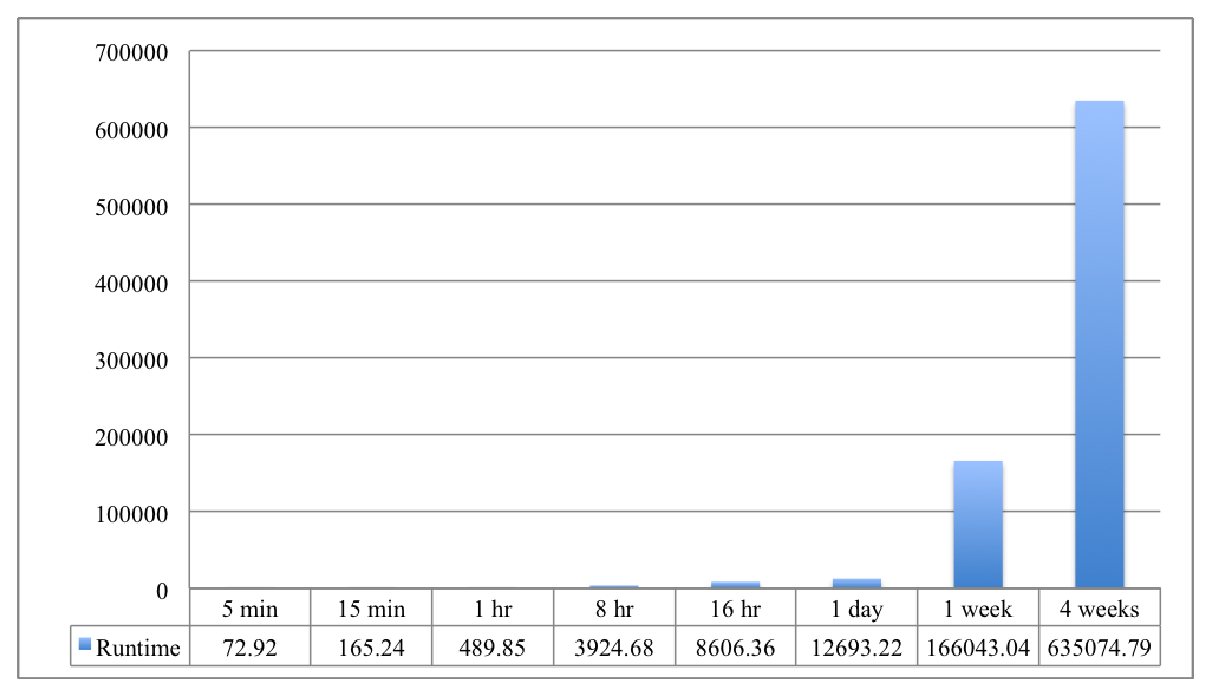
\includegraphics{runtime_different-epoch-spans_bar-table.eps}}
\rput(9.8,1.44){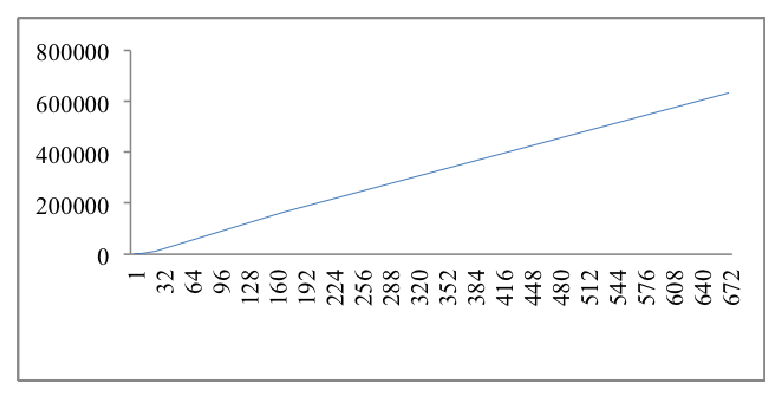
\includegraphics{runtime_different-epoch-spans_line.eps}}
\usefont{T1}{ptm}{m}{n}
\rput{90.15449}(0.96138316,-0.45039606){\rput(0.6871191,0.225){\LARGE Time in milliseconds}}
\usefont{T1}{ptm}{m}{n}
\rput(10.130039,-0.925){\Large Epoch span in hours}
\end{pspicture} 
}
\caption{Mean runtime at different epoch spans}
\label{fig:runtimeEpochs}
\end{figure}

\subsection{Mining Term N-grams}
\label{sec:ngrams}



\begin{figure*}[htb]
\centering
\scalebox{0.45} 
{
\begin{pspicture}(0,-3.56416)(37.82,3.5241601)
\usefont{T1}{ptm}{m}{n}
\rput(5.6938963,-3.2008398){\LARGE (a) Mean number of distinct items}
\usefont{T1}{ptm}{m}{n}
\rput(18.373896,-3.2008398){\LARGE (b) Mean number of itemsets}
\usefont{T1}{ptm}{m}{n}
\rput(32.033897,-3.2208397){\LARGE (c) Mean runtime in milliseconds}
\rput(5.93,0.50416017){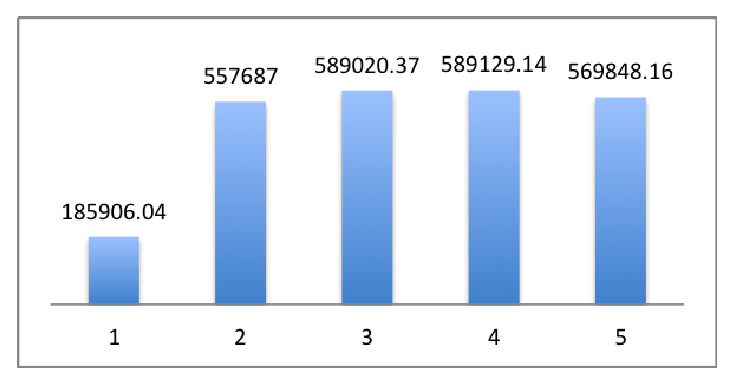
\includegraphics{perf_ngramlen1-5_distinct-items_supp10+_1hr.eps}}
\rput(18.89,0.5441601){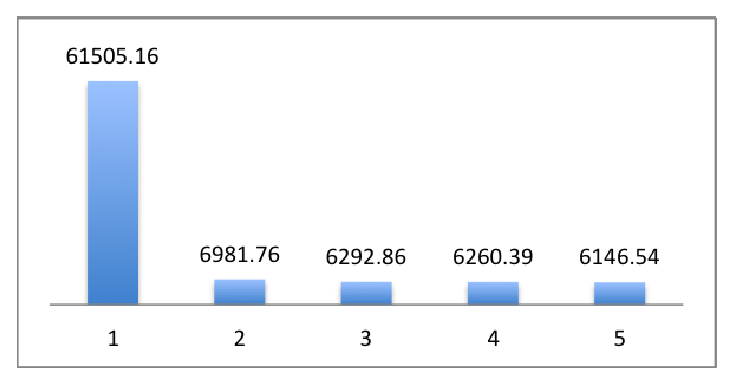
\includegraphics{perf_ngramlen1-5_itemsets_supp10+_1hr.eps}}
\rput(31.89,0.50416017){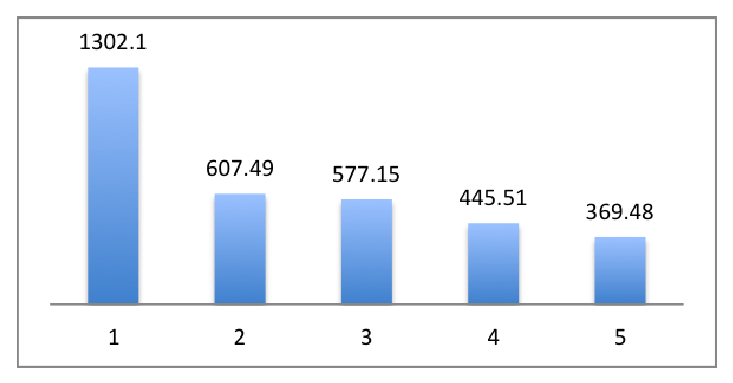
\includegraphics{perf_ngramlen1-5_runtime-millis_supp10+_1hr.eps}}
\end{pspicture} 
}
\caption{Effect of the increasing maximum N-Gram length on results of mining of 1hr epochs of data}
\label{fig:ngramsLen}
\end{figure*}


A large number of itemsets are language constructs that bear no information,
such as ``such as''. 
By treating sequential language constructs, and any other multiword expression,
as one item we eliminate a large number of such itemsets.
We can also eliminate itemsets that are made up of all the different fragments
of the language construct along with other items;
for example, \{we, did, it, \#teamobama\} can produce 10 other combinations of
length 2 or more.
There are many measures of association that can be used to detect multiword
expressions, but each measure is good only under certain conditions and has
special properties~\cite{ramisch2012broad}.
After preliminary experiments with various measures, we determined that
Yule's Q \cite{tan2002selecting} provides a reasonable method for
identifying multiword named entities.
Yule's Q is a measure of association and disassociation derived from the
odds ratio.
However, after further experimentation we determined that the best performance
could be obtained by tokenizing the documents into term N-grams with varying N. 

We start by tokenizing into unigrams, and counting their frequencies.
Then we use the probability of the same word used to determine the support
threshold, $P(`obama') = 0.0001$, and assume that this is where the head of
the Zipfean distribution starts.
For each unigram belonging to the head, we create two term bigrams by
attaching to it the unigrams before and after it.
We repeat this for each N $\ge$ 1 by creating two (N+1)-grams for all N-grams
with probabilities above the threshold until there are no more such N-grams.
We do not prevent overlap, because there is no guarantee that the N-Gram
created makes any sense.
At each N, the probability threshold is adjusted to account for the increase
in the number of tokens and the overall increase in the grand sum of counts,
since each high frequency N-Gram is replaced by two lower frequency ones.
Let the original probability threshold be $\eta$, then the adjusted $\eta_N$
is:
\begin{equation}\eta_N = \eta \times \frac{\sum_{\{w:\, w \,\in\, W\, and\, w.length \,\le\, N\}}{freq(w)}}{\sum_{\{v:\, v\, \in\, W \,and \,v.length\,=\,1\}}{freq(v)}}\end{equation}


Figure \ref{fig:ngramsLen} shows the effect of increasing the maximum length
of N-grams from 1 to 5 on the number of tokens, the number of closed itemsets
of length more than 1, and the runtime of mining one hour of data.
The values shown are averages across all one-hour epochs in the month of
November 2012.
The value of $\eta$ used is 0.0001.
Figure \ref{fig:ngramsLen}(a) shows that the number of distinct items
increases substantially as N goes from 1 to 2, then continues increasing
slightly until it starts decreasing at N=5.
The decrease happens because all 4-grams with probability above the threshold
are parts of tweets from services that use the same text and append a URL,
such as tweets reporting scores from
Game Insight\footnote{http://www.game-insight.com/}.
Such tweets are tokenized into more 4-grams than 5-grams, and the 4-grams
appearing in them do not appear elsewhere.
Thus, each pair is reduced to one 5-gram.
Figure \ref{fig:ngramsLen}(b) shows that the number of itemsets continues to
decrease as expected.
Figure \ref{fig:ngramsLen}(c) shows that runtime also decreases as N goes
from 1 to 5, since LCM runtime is proportional to the number of closed
itemsets, and is not affected by the sparsity of data.
The runtimes in this figure are slightly less from those in
figure \ref{fig:runtimeEpochs} because they do not include the time taken for
writing the posting list of each itemset.


After mining term N-grams we flatten the itemsets to sets of unigrams again.
This removes overlap between parts of itemsets making it easier to reason
about how they relate to each other. 
This is also necessary since an itemset will have different N-gram set
representations,
and its postings list is the union of those of the different representations.



\section{Filtering itemsets}
\label{sec:strong}


In the previous section, we discussed our handling of function words,
using a technique that exploits LCM's tolerance to sparsity.
After applying this technique, the average number of itemsets mined from an
hour of twitter data drops from 61,505 to 6,146.
However, there is still redundancy in the itemsets.

The closed property of an itemset is easily violated by modifying one
transaction that contains the itemset and removing one of its items.
While an update operation is not supported in the model of frequent itemsets
mining, a similar effect happens when people are writing about a certain fine
grained topic.
For example, figure \ref{fig:sham} illustrates  itemsets related to Donald
Trump's famous tweets in reaction to Obama's victory in
2012\footnote{http://www.huffingtonpost.com/2012/11/07/donald-trump-election-revolution\_n\_2085864.html}.  
Each area in the figure represents the transactions containing the itemset
formed by concatenating the items in all intersecting ellipses.  

The figure shows the effect of the lack of context and structure in
conversations happening on Twitter.
Because there was originally no way to refer to a certain tweet,
a tweet that sparked a conversation on Twitter had to be quoted in a retweet
along with the retweeter's comment.
This tradition still continues even though tweets can now explicitly reference
one another. 
Due to the 140 characters length limit of tweets the quotation usually has to
edited to be as short as possible by selecting only the most discriminative
words. 

In the figure, the most discriminative words are ``sham, and, travesty''
which are quoted along with Donald Trump's user name in most of the retweets.
Other people choose to also include ``not, democracy'' and/or ``elections'',
and in most of the cases the retweet indicator ``rt'' is added. 
This selection is an act of collaborative filtering,
but it results in many trivially different subsets from the original tweet.
The additions of retweeters also form many different supersets of the of the
original tweet, and some additions represent opinions that are supported
enough to be mined as itemsets. 

We propose two conditions that are not as easily violated as the closed
condition for selecting itemsets.
The two conditions build on the concept of \emph{association rule confidence}.
Confidence is the basic property used for association rules mining,
and it is used in the definition of $\delta$-free sets \cite{boulicaut2003free}.
Mining itemsets based on the confidence of rules they induce has long been
recognized as a method for finding
``interesting patterns'' \cite{cohen2001finding},
but since this property is not anti-monotone a variation has to be used
(for example, \emph{all confidence} \cite{kim2004ccmine}).
The confidence of an assocation rule that the presence of an itemset,
$s_{j}$, implies the presence of another itemset, $s_i$, is  defined as:
\begin{equation}\label{eq:conf}conf(s_j \rightarrow s_i) = \frac{|T_{s_i} \cap T_{s_j}|}{|T_{s_j}|}\end{equation}


\begin{figure}
\centering
%\scalebox{0.7} 
\resizebox{7cm}{3.5cm}
{
\begin{pspicture}(0,-2.649212)(9.077745,2.95)
\psframe[linewidth=0.04,dimen=outer](8.843161,2.95)(0.2431605,-2.61)
\usefont{T1}{ptm}{m}{n}
\rput(4.103317,1.675){sham, and, travesty}
\usefont{T1}{ptm}{m}{n}
\rput(1.7484828,2.575){@realdonaldtrump}
\pscircle[linewidth=0.04,dimen=outer](4.1031604,0.01){2.28}
\rput{55.644855}(2.9522903,-5.6005197){\psellipse[linewidth=0.04,dimen=outer](6.782275,-0.0031560312)(1.9103949,2.0626228)}
\rput{34.21703}(0.13301769,-1.7201583){\psellipse[linewidth=0.04,dimen=outer](2.8607624,-0.6440031)(2.908739,0.81)}
\pscircle[linewidth=0.04,dimen=outer](4.5031605,-0.33){1.58}
\usefont{T1}{ptm}{m}{n}
\rput(4.527965,-0.865){not,}
\pscircle[linewidth=0.04,linestyle=dashed,dash=0.16cm 0.16cm,dimen=outer](2.6031604,0.81){0.48}
\usefont{T1}{ptm}{m}{n}
\rput(1.0566566,1.455){fraud}
\pscircle[linewidth=0.04,linestyle=dashed,dash=0.16cm 0.16cm,dimen=outer](1.0631605,1.45){0.46}
\usefont{T1}{ptm}{m}{n}
\rput(2.623102,0.815){hair}
\pscircle[linewidth=0.04,dimen=outer](7.3231606,-1.35){1.02}
\usefont{T1}{ptm}{m}{n}
\rput(7.337262,-1.025){the, world, }
\usefont{T1}{ptm}{m}{n}
\rput(7.264635,-1.325){is, laughing}
\rput{34.21703}(0.8391447,-4.3701773){\psellipse[linewidth=0.04,dimen=outer](7.5185595,-0.8219682)(1.3607179,0.95923364)}
\rput{34.21703}(0.3818179,-4.274056){\psellipse[linewidth=0.04,dimen=outer](7.133755,-1.5167968)(1.2777647,0.86427283)}
\usefont{T1}{ptm}{m}{n}
\rput(7.207018,-1.645){at}
\usefont{T1}{ptm}{m}{n}
\rput(8.076705,-0.165){us}
\usefont{T1}{ptm}{m}{n}
\rput(6.371842,-2.105){you}
\usefont{T1}{ptm}{m}{n}
\rput(1.4102015,-1.625){elections}
\usefont{T1}{ptm}{m}{n}
\rput(6.9122915,1.255){rt}
\usefont{T1}{ptm}{m}{n}
\rput(4.4461293,-1.265){democracy}
\end{pspicture} 
}

\caption{Closed, distinct and strongly closed sets}
\label{fig:sham}
\end{figure}


\begin{algorithm}
\SetAlgoLined
\LinesNumbered
\KwIn{$\kappa$: Minimum distinctiveness threshold} 
\KwData{$\mathcal{C}$: Closed Itemsets produced by LCM}
\KwResult{$\mathcal{R}$: Strong closed itemset clusters}
\For{$i \gets 2$ to $|\mathcal{C}|$}{
	$C \gets \{s_c: s_c \in \mathcal{C} \, and \, c < i \, and \, |s_c \cap s_i| > 0\}$\;
	$P \gets \{s_p: s_p \in \mathcal{C} \, and \, p < i \, and \, s_p \cap s_i = s_i\}$\;
	$s_p \gets \textbf{argmax}_{s_p \in P}\frac{|T_{s_i}|}{|T_{s_p}|}$ \tcp*{Direct parent}
	\uIf{$\frac{|T_{s_i}|}{|T_{s_p}|} < \kappa$}{continue\tcp*{Not a distinct itemset}}
	$s_m \gets s_i$  \tcp*{Cluster centroid, initially self}
	$maxConf \gets 0$ \tcp*{Best candidate's score}
	\ForEach{$s_c \in C$}{
		$\Delta \gets (1 - (1-\kappa)) |T_{s_c}|$ \tcp*{Maximum difference}
		$\delta \gets$ difference($T_{s_c},T_{s_c \cup s_i},\Delta$) \tcp*{Stops early}
		
		\If{$\delta \le \Delta$}{ 
			$conf \gets \frac{|T_{s_c}| - \delta}{ |T_{s_c}|}$\;
			\If{$conf > maxConf$}{
				$s_m \gets s_k$ \tcp*{Best merge candidate}
				$maxConf \gets conf$ \;
			}
		}
	}
	$\mathcal{R}[s_i] \gets \mathcal{R}[s_m]$ \tcp*{Cluster $s_i$ with $s_m$}
	$\mathcal{R}[s_m].itemset \gets \mathcal{R}[s_m].itemset \cup s_i \cup s_m$\;
	$\mathcal{R}[s_m].postingsList \gets \mathcal{R}[s_m].postingsList \cup s_i.postingsList \cup s_m.postingsList$\;
}
\Return{$\mathcal{R}$}\;
\caption{Forming strong closed itemset clusters}
\label{algo:alliance}
\end{algorithm}

\subsection{Distinct Itemsets}


The \emph{distinct} condition is a novel strengthening of the closed condition
so that it is not violated by trivial differences.
We define a \emph{distinct} itemset as a closed itemset whose frequency
comprises more than a certain proportion of the frequency of its least
frequent subset. 
This condition chooses closed itemsets which substantially violate the closed
condition of their subsets.
The proportion is a parameter, $\kappa$, that controls the selectivity of the
\emph{distinctiveness} condition.
This can be interpreted as selecting itemsets which are implied by a subset
with confidence greater than $\kappa$.
Formally, the set of \emph{distinct} itemsets, $\mathcal{D}$,
is defined as follows:
\begin{equation}\mathcal{D} = \{s: s \in \mathcal{C} \, and \, \exists \; s_{p} \subset s \; where \; \frac{|T_{s}|}{|T_{s_{p}}|} \ge \kappa 
\}\end{equation}

In figure \ref{fig:sham}, \emph{distinct} itemsets are illustrated in solid
lines, and closed itemsets that do not satisfy the distinctiveness condition in dashed lines.
It is clear from the figure that considerable redundancy remains in
\emph{distinct} itemsets.

\subsection{Strongly Closed Itemsets}
To remove the redundancy in \emph{distinct} itemsets we merge similar ones
into \emph{strongly closed} itemset clusters.
The similarity of a \emph{distinct} itemset,
$s_d$, and another distinct itemset, $s_c$,
is measured as the overlap of the \emph{transactions} containing both of them
with the transactions containing $s_c$. 
A \emph{distinct} itemset is clustered with another itemset if one exists
such that the overlap exceeds a similarity threshold,
which we take to be $1-\kappa$ (the indistinctiveness of $s_d$ from $s_c$).
If more than one satisfies this condition,
the  \emph{distinct} itemset is clustered with the one having the highest
overlap ratio.
When  a \emph{distinct} itemset is clustered with an itemset that is already
part of a cluster, the \emph{distinct} itemset is added to the existing cluster.
Finally, the \emph{strongly closed} itemset is the union of all cluster members,
and its support is the size of the union of their postings lists.
We define the  desired clustering  and the strongly closed itemset
represented by each cluster as follows:
\begin{align*}\label{eq:strongClosedFormal}
\mathcal{R} = \{r: r = \bigcup_i{(s_i, s_j)}\; where\; s_i \in \mathcal{D} \, and \, s_j \in \mathcal{D} 
\\\,and\; \forall_{(s_i,s_j)} \, s_j = \textbf{argmax}_{s_k} conf(s_k \rightarrow s_i) \\\,and \;conf(s_j \rightarrow s_i) \ge (1-\kappa)
\\\, and\;( s_j = r.centroid\; or \; (s_j, r.centroid) \in r )\}
\end{align*}
\begin{equation}S_l = \{w:\, w \in \bigcup_{(s_i, s_j) \in r_l}{s_i} \; where \; r_l \in \mathcal{R}\}\end{equation}

This clustering scheme selects the cluster that contains the itemset which
maximizes the confidence of the rule $conf(s_j \rightarrow s_i)$,
with a lower bound on the overlap to maintain distinctiveness. 
This clustering can be implemented efficiently using techniques similar to
the ones proposed by Bayardo et al. \cite{bayardo2007scaling}.
The main ideas are to limit the comparisons to a few candidates,
and to terminate the comparison early if the similarity threshold will not
be met.
In our case, the postings lists are longer than the itemsets,
so we generate candidates for comparison by calculating similarity between
itemsets.
When calculating the similarity between two postings lists,
we can terminate early if the difference exceeds the maximum difference
permissible to achieve a similarity of $1-\kappa$,
which can be derived from equation \ref{eq:conf}. 

Algorithm~\ref{algo:alliance}  shows a possible implementation.
For each itemset, $s_i$, we find the itemsets produced before it
and overlapping with it in one or more items.
Then we find the candidate, $s_c$, that maximizes
$conf(s_c \rightarrow s_i)$ such that the confidence exceeds $1-\kappa$.
Notice that confidence is not a symmetric measure,
and we only check the confidence of the rule that the clustering candidate
implies the itemset. 

\subsection{Performance Analysis}
\label{sec:bounding}
We analyze the performance of the filtering conditions proposed by applying
them to the mining results of all one-hour long epochs in the Twitter data.
The average number of itemsets mined from an hour-long epoch is
2439.17 closed itemsets of length 2 or more;
that is, excluding itemsets that are merely a frequent item.
The number of length 2 or more maximal itemsets is 1831.92,
which we provide just as a reference to the result of a basic way of filtering.

Figure \ref{fig:kappa} show the effect of varying $\kappa$ on the mean number
of \emph{distinct} and \emph{strong closed} itemsets.
The number of \emph{distinct} itemsets drops as the distinctiveness threshold
increases.
On the other hand, the number of \emph{strong closed} clusters formed increases
as the similarity (indistinctiveness) threshold decreases.
The dashed line shows that the number of unclustered distinct itemsets reaches
zero at $\kappa=0.5$, explaining why the number of clusters changes very
slightly after that. 
We use $\kappa = 0.25$ in the remainder of the paper,
which is an arbitrary choice based on the definition not the data.
The average number of itemsets (\emph{strongly closed} and unclustered
\emph{distinct}) mined from one-hour epochs at this value of
$\kappa$ is only 224.48 which is about 10\% of the number of closed itemsets.

\begin{figure}
\scalebox{.5} 
{
\begin{pspicture}(0,-4.16)(16.6,4.16)
\rput(8.3,0.0){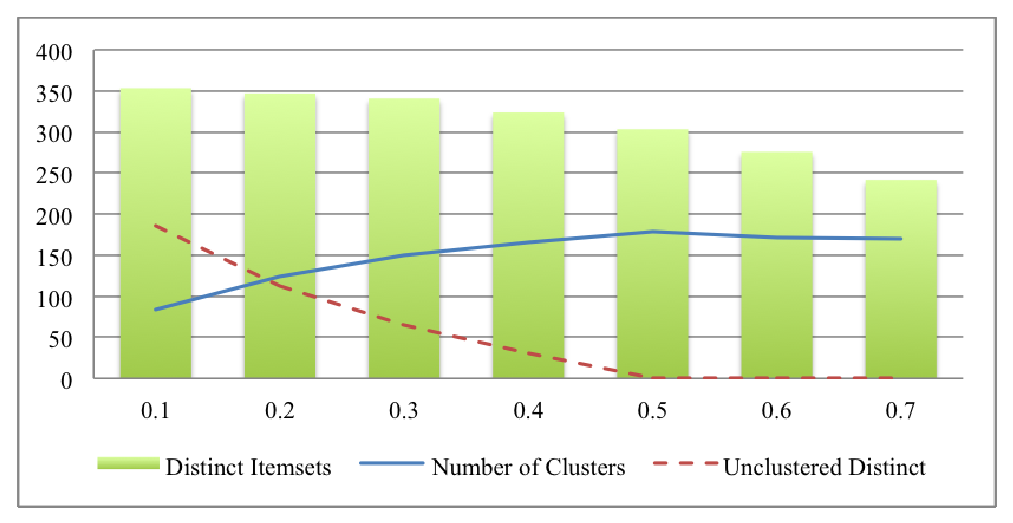
\includegraphics{kappa_effect.eps}}
\end{pspicture} 
}
\caption{Effect of changing $\kappa$ on mining results }
\label{fig:kappa}
\end{figure}



Figure \ref{fig:lcmvsfpzhu} shows the total runtime of the LCM algorithm plus
filtering based on the distinct condition and clustering into strong closed
itemsets at different epoch spans.
The runtime of LCM alone is also plotted for reference.
We also plot the performance of another frequent itemset mining algorithm,
FP-Zhu \cite{grahne2004reducing}, which was the runner up at
FIMI 2004~\cite{DBLP:conf/fimi/2004}.
We include it to show that our extensions do not degrade the performance of
LCM even in the context of competitions.
The y-Axis is in logarithmic scale to keep the scale of the plot suitable for
seeing slight differences.
The output of LCM is the input to the filtering and clustering step,
so it is affected by the number of closed itemsets produced.
This explains why it takes slightly longer time for clustering results from
the 15-minute epoch and then takes a constant time for epochs of longer span. 

The experiments were run using a single threaded Java implementation of
algorithm \ref{algo:alliance}.
The experiments were run on a 1.4GHz processor with 2MB of cache.
Unlike the original LCM algorithm, filtering low confidence itemsets requires
us to keep mined results in memory to calculate the confidence of newly
generated ones.
The memory requirement is not large because the number of itemsets averages
at about 6000.
In our experience with the Twitter data it was enough to keep only a buffer
of 1000 itemsets, and this is what we use for the runtime performance
evaluation and the empirical evaluation of the filtering results in
sections \ref{sec:empirical}.
If all itemsets are kept in memory the runtime increases slightly and
averages at 5.2 seconds for filtering a one-hour epoch.



\begin{figure}
\centering
\resizebox{9cm}{4.25cm}
%\scalebox{0.6} % Change this value to rescale the drawing.
{
\begin{pspicture}(0,-4.52)(16.408476,4.52)
\rput(7.52,0.0){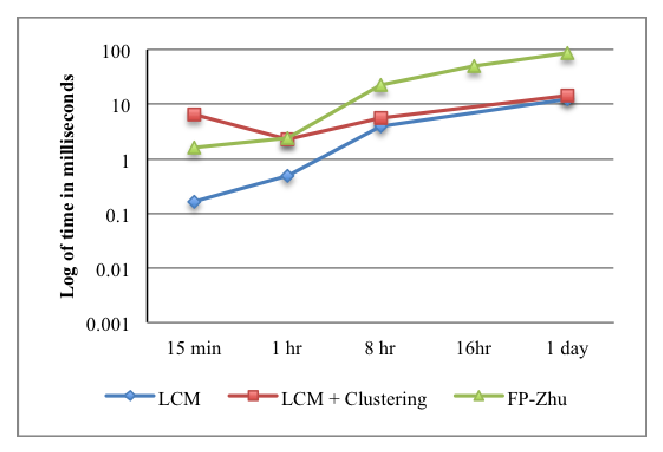
\includegraphics{runtime_lcm-lcm+filter-fpzhu_seconds.eps}}
\usefont{T1}{ptm}{m}{n}
\rput(14.1,-3.85){\large ($\kappa = 0.25$)}
\end{pspicture} 
}
\caption{Runtime of itemset mining alone and with filtering and clustering at different epoch spans}
\label{fig:lcmvsfpzhu}
\end{figure}


\section{Temporal Ranking}
\label{sec:rank}
The previous filtering steps reduce the number of itemsets to under 1\% of their
original numbers.
In this section, we present a method for ranking itemset clusters according to
their novelty when compared to other time periods.
These itemsets can then be presented to users in rank order, providing a
synopis of events in the epoch, or used as input to additional search or
summarization steps.

A good indicator of novelty is the pointwise Kullback-Leibler Divergence (KLD)
between an itemset's probability in the current epoch and in a longer past
epoch~---~the background model.
The pointwise KLD of the probability of an itemset $s_i$ in the background
model $Q$ from its probability in the current epoch $P$ can be considered as
the information gain, IG: 
\begin{align}IG(P(s_i),Q(s_i))  = - (H(P(s_i)) - H(P(s_i),Q(s_i))) \notag\\ = \sum{P(s_i) \log{P(s_i)}} - \sum{P(s_i) \log{Q(s_i)}} \notag\\ = KLD(P(s_i)||Q(s_i))\end{align}

To generalized this formula to the case of strongly closed itemset clusters,
we have to take the overlap between the itemsets of the cluster into account
when calculating the information gain of the whole cluster.
We note that the joint probability of the itemset, $s_i$, and its superset,
$s_j$, is equal to the probability of the superset;
$P(s_i,s_j) = P(s_j)$ and $Q(s_i,s_j) = Q(s_j)$. 
Thus, the information gain of the appearance of an itemset and its superset
together is essentially the information gain of the superset;
$IG(P(s_i,s_j),Q(s_i,s_j)) = IG(P(s_j),Q(s_j))$.
Also, their pointwise mutual information (PMI) is the self information (SI) of
the subset:
\begin{align}
PMI(s_i, s_j) = \log{ \frac{P(s_i,s_j)}{P(s_i)P(s_j)} } = -\log{P(s_i)} = SI(s_i)
\end{align}

Therefore, the information gain of a superset is different from the
information gain of its subset by the information gained (or lost) because
of the additional items.
Hence, the information gain of a strong closed itemset cluster,
$S=\{s_{i1},..,s_{im}\}$, 
can be approximated as the information gain of its smallest subset, $s_{min}$,
plus the differences between the IGs of member subsets and the smallest subset.
We use the squares of the differences, because the IG value can be positive or
negative, and we only care about the magnitude of the difference.
To give the self information of the smallest subset the same influence,
we also square it.
Thus, the information gain of a strong closed itemset is given by:
\begin{multline}IG^2(P(s_{i1},...s_{im}),Q(s_{i1},...s_{im})) =\notag\\ I^2(s_{min}) + \notag\\ 
\sum_{j = i1..im}{(IG(P(s_j)||Q(s_j)) - IG(P(s_{min})||Q(s_{min})))^{2}} \end{multline}

The formula above can be used directly for ranking clusters,
but it will favour larger ones.
We normalize by the size of the cluster giving our final ranking formula for
strong closed itemsets:
\begin{equation}\label{eq:avgIG}\overline{IG}(S) = \frac{IG^2(P(s_{i1},...s_{im}),Q(s_{i1},...s_{im}))}{m}\end{equation}


\subsection{Empirical Evaluation}
\label{sec:empirical}
We now show examples of the performance the proposed methods in creating
a synopses of the 2012 election day, November $6^{th}$, and another less
eventful day, November $9^{th}$.
The background model we use for each day is the results of mining the 4 weeks
before it, using a \emph{minimum support} value of 1 occurrence.
Mining the background model at such a low support increases the number of
produced itemsets, which is desirable for a background model.
All probability estimates are smoothed by add-one smoothing. 

Tables \ref{table:nov6} and \ref{table:nov9}  show the top 3 itemsets for
one-hour epochs in the days examined.
The itemsets shown are the first appearances of the most interesting itemsets;
that is, an hour is shown only if its top 3 feature novel interesting itemsets. The first column is the beginning of the hour, EST time.
The second column is the top itemsets.
The third column is a commentary to explain the itemsets,
but we omit it from table \ref{table:nov9} to save space since the itemsets are self explanatory.

In table \ref{table:nov6}, we can see how the events of the US presidential
elections  unwind from ``get out and vote'' to the projections and debates,
all the way to the ``acceptance speech''.
Early in the day, itemsets about UEFA Champions football matches and a TV show
``Geordie Shore'' appear in the top 3 along with itemsets about the still
uneventful elections.
Actually, the matches keep occupying top positions and timely updates of their
scores appear in the top 30 itemsets, until they end and the elections
heats up.
Shortly after the results of the elections became clear, news that
``weed is legal in Colorado'' occupies the top position.
This exemplifies the power of social media as a collaborative filter,
selecting the news of greatest importance to social media users.
The user centric definition of importance is also evident in attention
given to the ``lady behind Obama  with a flag in her hair'' during the
acceptance speech. 

On November $9^{th}$, table \ref{table:nov9}, the most interesting hour is
15:00.
The MTV Europe Music Awards (MTVEMA) was taking place and votes were solicited
from the audience through Twitter.
This is an example of a topic where people have strongly different opinions.
The top 3 itemsets of the hour 15:00 are supporting ``Katy  Perry'',
``Justin Bieber'' and ``Lady Gaga'' respectively.
They are all reported as separate itemsets, showing how clustering using the
postings lists avoid forming incohesive clusters.
No other major events were happening but many overlapping minor ones happened.
The day started by news about the end of two careers;
the Laker's ``coach Mike Brown'' got fired  and ``CIA director David Petraeus
resigns''.
A personal relationship of Justin Bieber also ends as he
``broke, up, with, Selena, Gomez'' at 22:00.
This event overlaps with his participation in the MTVEMA,
and both topics occupied high (but distinct) rankings. 
By the end of the day in North America, many congratulations for the
Indonesian Hero's day (``Hari Pahlawan'') appear, and the Turkish
commemoration day of Ataturk is also mentioned as the 10th of November has
started in these countries.
These are examples of itemsets from languages with a relatively low number of
users, showing how the absolute popularity of a topic does not affect its rank.
If itemsets from only a specific language is desired,
language identification can be applied on the itemsets and tweets from their
postings lists.
Moving language identification downstream avoids affecting the results of
mining because of error in an upstream component.

\begin{table}

\begin{center}
\small
\def\arraystretch{1.1}
\begin{tabular}{|p{.6cm}|p{2.5cm}|p{5cm}|}

\hline
\multirow{3}{*}{\texttt{13:00}} 	&  0, 1, de, jong 			& De Jong scores for Ajax \\ \cline{2-3} %http://www.dailymail.co.uk/sport/football/article-2228815/Manchester-City-2-Ajax-2--match-report-Siem-Jong-Yaya-Toure-Sergio-Aguero-Champions-League.html
					   	& geordie, shore		& Season 5 of the TV series starts \\ \cline{2-3}
						& get, out, and, vote		& Still early in the U.S. elections day \\\hline

\multirow{3}{*}{\texttt{17:00}} 	&  if, obama, wins		& Speculations regarding elections \\ \cline{2-3}
					   	& USERNAME, spots, my, club		&  Pyramidal marketing scam. Retweeted by people to make money.  \\ \cline{2-3}
						& the, polls, close		& Polls to start closing at 6 PM \\\hline %http://www.huffingtonpost.com/2012/11/06/what-time-do-polls-close_n_2080894.html

\multirow{3}{*}{\texttt{19:00}} 	&  A partir de que idade voc\^{e} considera algu\'{e}m velho?		& Internet meme from Brazil, discussing when to start considering a person old. \\ \cline{2-3}
					   	& food, stamps		& Discussions pertaining to elections \\ \cline{2-3}
						& linda, mcmahon, senate		&  Linda McMahon loses CT senate race \\\hline

\multirow{3}{*}{\texttt{20:00}} 	& obama, got, this		&  Announcing states that Obama got \\ \cline{2-3}
					   	& projected, winner		& Early projections about who will win \\ \cline{2-3}
						& moving, to, canada		&  Reaction to projections \\\hline


\multirow{3}{*}{\texttt{21:00}} 	& elizabeth, warren		&  MA senate elections winner \\ \cline{2-3}
					   	& popular, vote		& Comparing Popular vs Electoral votes \\ \cline{2-3}
						& who, is, the, president?		&  Anticipation for the elections results\\\hline
						

\multirow{3}{*}{\texttt{22:00}} 	& \#forward, \#obama2012		&  Obama won, time to move \#forward \\ \cline{2-3}
					   	& my, president, is, still		& Some were saying Black (skin colour), others Blue (party colour) \\ \cline{2-3}
						& back, in, office		&   Obama is back in office\\\hline

\multirow{3}{*}{\texttt{22:30}} 	& once, you, go, black		& A popular cultural reference.\\ \cline{2-3} %  .. you never go back. 
					   	& @realdonaldtrump, this, elections, ... [his famous tweet] 		& Donald Trump is a Republican and he could not accept Obama's victory\\ \cline{2-3}
						& concession, speech, write		&   The losing candidate has to concede before the winner declares victory \\\hline
						
\multirow{3}{*}{\texttt{23:00}} 	& weed, is, legal, in, colorado		&  This piece of news got the attention as soon as it was announced  \\ \cline{2-3}
					   	& karl, rove		& Fox news challenges results from Ohio\\ \cline{2-3}
						& our, country, is, trouble		&   Dramatic reactions to elections \\\hline						
\multirow{3}{*}{\texttt{23:30}} 	& acceptance, speech, wrote		&  Obama wrote his speech, ...\\ \cline{2-3}
					   	& give, his, speech		& ... and is going to deliver it ... \\ \cline{2-3}
						& on, cnn		&   ... on CNN. \\\hline	
						
\multirow{3}{*}{\texttt{00:30}} 	& behind, obama, with, flag, in, her [hair]		&  During the speech, attention on social media goes to a woman appearing behind Obama on TV! \\ \cline{2-3}
					   	& the, best, is, yet, to, come		&  Quote from Obama's speech\\ \cline{2-3}
						& flag, that, weaves	& Play on words about the ``flag in hair'' \\\hline																			
\end{tabular}
\end{center}
\caption{Top 3 itemsets for hours in November 6th}
 \label{table:nov6}
\end{table}

\begin{table}

\begin{center}
\small
\def\arraystretch{1.1}
\begin{tabular}{|p{.6cm}|p{7.5cm}|}

\hline
\multirow{3}{*}{\texttt{12:00}} 
& \#iwillneverunderstand, why\\\cline{2-2}
& breaking, news, head, coach, mike, brown, have, fired  \\\cline{2-2}
& USERNAME, spots, available, my, club \\\hline
\multirow{3}{*}{\texttt{14:00}} 
& cia, director, david, petraeus, resigns \\\cline{2-2}
& voc\^{e}, acha, que \\\cline{2-2}
& \#tvoh [the voice of Holland], babette \\\hline
\multirow{3}{*}{\texttt{15:00}} & \#emawinkaty, i, think, katy, perry, will, be, the, big,  \#mtvema, winner, tweet, your, pick, at, URL
\\ \cline{2-2}
& \#emawinbieber, i, think, justin, bieber, ... [same as above] \\ \cline{2-2}
& \#emawingaga, ... [same as above]  \\\hline														
\multirow{3}{*}{\texttt{22:00}} & justin, bieber, and, selena, gomez, broke, up
\\ \cline{2-2}
& selamat, hari, pahlawan \\\cline{2-2}
& aniyoruz, kemal, mustafa [ataturk] \\ \hline
\end{tabular}
\end{center}
\caption{Top 3 itemsets for hours in November 9th}
 \label{table:nov9}
\end{table}
 
 

\section{Conclusion and future work}
\label{sec:concfut}
We have proposed a method for efficiently creating temporal synposes of social
media streams, based on a frequent itemset mining algorithm that is suitable
for sparse data, LCM.
Our method summarizes an hour of Twitter data (100,000 tweets on average) into
224 itemsets in 1945.68 milliseconds on average,
and scales for longer epochs of data.
The direct application of LCM on one-hour epochs of Twitter data results in
an average of 61505.16 closed itemsets and takes 2506.58 milliseconds on
average.
The improvement is due to the following contributions: 
(1) strengthening  the closure condition such that it selects an itemset only if
it is distinctively different from its subsets and other itemsets, and 
(2) using variable length N-grams to mitigate the effect
of the skewness of the frequency distribution of unigrams.
The distinctiveness between two itemsets is based on a parameter, $\kappa$, which controls tolerance to redundancy. %Even though the use or variable length N-grams

Another important contribution is a method for ranking itemsets based on their temporal novelty.
The top 3 itemsets from the hours of election day and another less eventful
day shows that the synopses captures important events, and might reasonably
be directly presented to users as a summary.
A possible future direction is to use itemsets that appear as a sequence for
building extractive coherent summaries of the social media stream at
different times.

We aim to exploit the synopses for temporal query expansion in our future work. Terms from itemsets relevant to a query (or occurring in a relevant document)
can be used for query expansion, thus acting as precomputed results of 
pseudo-revelance feedback.
We also wish to explore ways to make use of the temporal signal during mining,
such as when calculating similarity during clustering.

 

%\section{Acknowledgements}
% No Acknowledgments yet...
%This paper was funded in part by the Google Focus Award. Right?? What else should we say here? I am writing to fill some space and reserve it for the actual acknowledgements.
%% Thank YOU!



% The following two commands are all you need in the
% initial runs of your .tex file to
% produce the bibliography for the citations in your paper.
\bibliographystyle{abbrv}
\bibliography{younos_cikm2013}  % sigproc.bib is the name of the Bibliography in this case
% You must have a proper ".bib" file
%  and remember to run:
% latex bibtex latex latex
% to resolve all references
%
% ACM needs 'a single self-contained file'!
%
%APPENDICES are optional
%\balancecolumns

\end{document}
